% This LaTeX document needs to be compiled with XeLaTeX.
\documentclass[12pt]{article}
\usepackage[margin=0.8in]{geometry}
\usepackage[utf8]{inputenc}
\usepackage{graphicx}
\usepackage[export]{adjustbox}
\usepackage{amsmath}
\usepackage{amsfonts}
\usepackage{amssymb}
\usepackage[version=4]{mhchem}
\usepackage{stmaryrd}
\usepackage{bbold}
%\usepackage[fallback]{xeCJK}
\usepackage{polyglossia}
\usepackage{fontspec}
\usepackage{censor}
%\setCJKmainfont{Noto Serif CJK TC}
\graphicspath{ {../Images/} }
\usepackage{enumitem}
\usepackage{tikz}
\usepackage{amsthm}
\usepackage{tcolorbox}
\usepackage{array}
\usepackage{tabularray}
\usepackage{makecell}

\tcbuselibrary{theorems}

\definecolor{GrayCen}{HTML}{d2d2d2}
\definecolor{GrayBG}{HTML}{d9d9d9}
\definecolor{BlueDef}{HTML}{104e8b}
\definecolor{GreenProp}{HTML}{025540}
\definecolor{RedMet}{HTML}{cd5556}
\definecolor{BlackSav}{HTML}{000000}
\def\censorcolor{GrayCen}
\let\svcensorrule\censorrule
\renewcommand\censorrule[1]{%
\textcolor{\censorcolor}{\svcensorrule{#1}}}

\newtcbtheorem
  []% init options
  {definition}% name
  {Définition}% title
  {%
    colback=GrayBG,
    colframe=BlueDef,
    fonttitle=\bfseries,
  }% options
  {def}% prefix

\newtcbtheorem
  []% init options
  {proposition}% name
  {Proposition}% title
  {%
    colback=GrayBG,
    colframe=GreenProp,
    fonttitle=\bfseries,
  }% options
  {prop}% prefix

\newtcbtheorem
  []% init options
  {method}% name
  {Méthode}% title
  {%
    theorem name,
    colback=GrayBG,
    colframe=RedMet,
    fonttitle=\bfseries,
  }% options
  {met}% prefix
  
\newtcbtheorem
  []% init options
  {savoir}% name
  {Savoir-faire du chapitre}% title
  {%
    theorem name,
    colback=GrayBG,
    colframe=BlackSav,
    fonttitle=\bfseries,
  }% options
  {sav}% prefix

\newtheoremstyle{break}
  {\topsep}{\topsep}%
  {}{}%
  {\bfseries}{}%
  {\newline}{}%
\theoremstyle{break}
\newtheorem*{example}{Exemple.}
\newtheorem*{remark}{Remarque.}

\newenvironment{demo}[1][\proofname]{%
  \begin{proof}[#1]$ $\newline
}{%
  \end{proof}
}

\setmainlanguage{french}
%\setmainfont{CMU Serif}

\title{
\vspace{4em}
\centering
\tcbset{colframe=BlackSav,colback=GrayBG}
\tcbox[tikznode]{
Chapitre 6 \\Trigonométrie
}
}

\author{}
\date{}

\setlength\parindent{0pt}
%\setlist[itemize]{topsep=0pt}
\setlist{nolistsep}
%\setlist[itemize]{noitemsep}
%\setlist[enumerate]{noitemsep}


\newcolumntype{C}[1]{>{\centering\arraybackslash}m{#1}}
\newcolumntype{L}[1]{>{\raggedright\arraybackslash}m{#1}}
\newcolumntype{N}{@{}m{0pt}@{}}

\begin{document}
\maketitle

\tableofcontents

%\newcommand{\hideM}[1]{\mbox{\vphantom{$#1$}\smash{\colorbox{gray!50}{$\displaystyle #1$}}} }
%\newcommand{\hide}[1]{\mbox{\vphantom{#1}\smash{\colorbox{gray!50}{#1}}}}
\newcommand{\hideM}[1]{\mbox{\vphantom{$#1$}\smash{\colorbox{gray!50}{\phantom{$\displaystyle #1$}}}} }
\newcommand{\hide}[1]{\mbox{\vphantom{#1}\smash{\colorbox{gray!50}{\phantom{#1}}}}}

\newpage 
\section{Cercle trigonométrique et repérage d'un point}
\subsection{Cercle trigonométrique}
\begin{definition}{}{}
Dans un repère orthonormé ( $\mathrm{O} ; \mathrm{I}, \mathrm{J}$ ), le \hide{\textbf{cercle trigonométrique}} $\mathcal{C}$ est le cercle de centre \hide{O} et de rayon \hide{1}, parcouru dans le sens inverse des aiguilles d'une montre, appelé \hide{\textbf{sens direct}} ou encore \hide{\textbf{sens trigonométrique}}.
\end{definition}
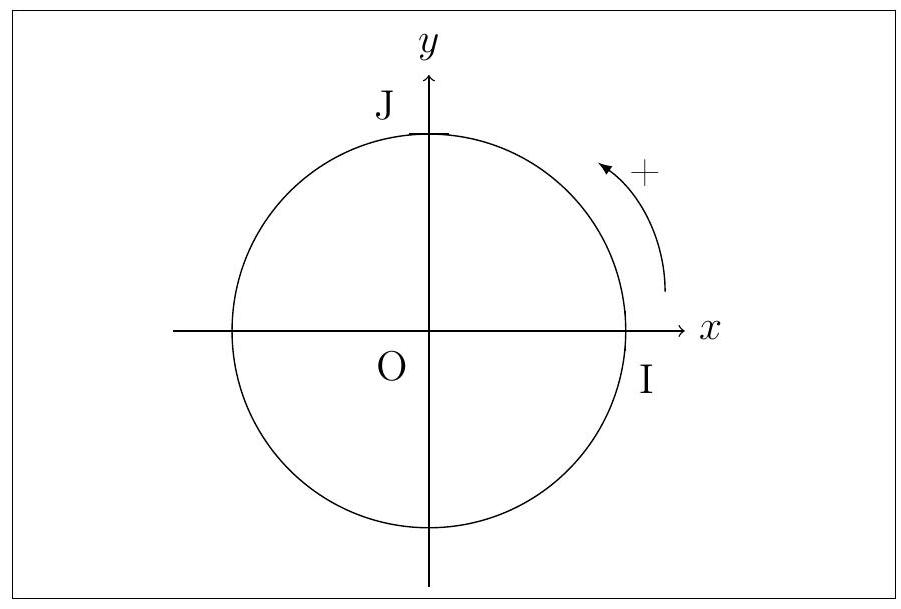
\includegraphics[width=0.45\textwidth, center]{2024_12_30_08b7afd589db230261ebg-02}

\subsection{Repérage sur le cercle trigonométrique}
\begin{remark}
On place la droite numérique perpendiculaire à (OI) telle que le 0 de la droite numérique coïncide avec le point I et on l'oriente dans le sens de O vers J (vers le haut). On enroule la demi-droite des réels positifs sur le cercle $\mathcal{C}$ dans le sens trigonométrique et la demi-droite des réels négatifs sur le cercle $\mathcal{C}$ dans le sens indirect.

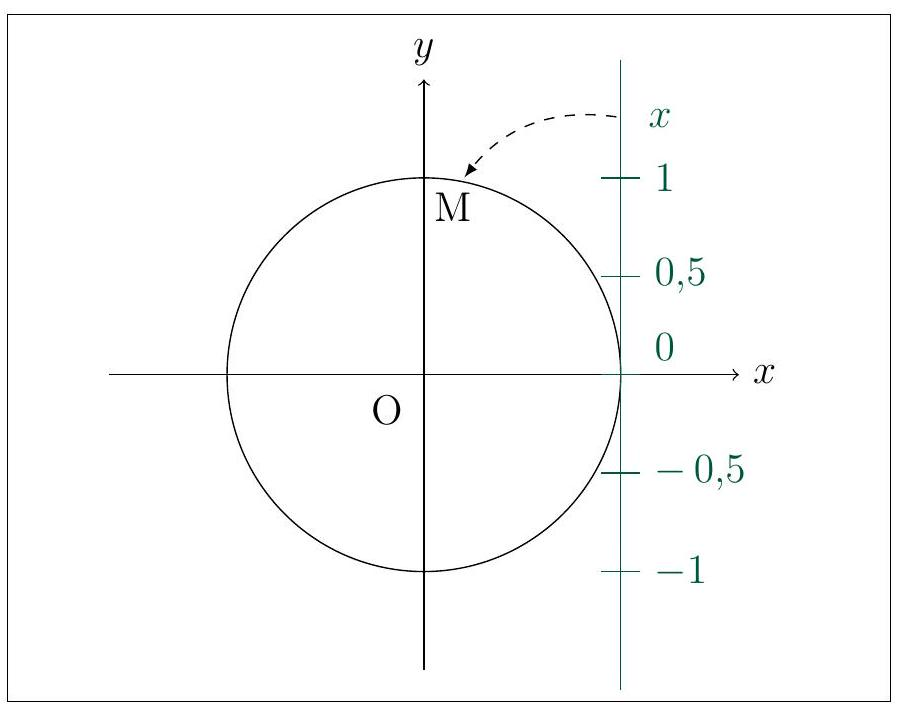
\includegraphics[width=0.45\textwidth, center]{2024_12_30_08b7afd589db230261ebg-02(1)}
\end{remark}

\begin{definition}{}{}
À chaque nombre réel $x$ de la droite numérique, on associe un unique point M du cercle trigonométrique que l'on appelle \hide{\textbf{point image}} de $x$.
\end{definition}

\begin{proposition}{}{}
Deux nombres réels $x_{1}$ et $x_{2}$ ont le même point image sur $\mathcal{C}$ si, et seulement si, il existe $k \in \mathbb{Z}$ tel que :

$$
x_{2}=x_{1}+\hideM{k \times 2 \pi}
$$
\end{proposition}

\begin{demo}
Soit M un point du cercle trigonométrique. Les nombres réels ayant pour point image M sont obtenus en parcourant l'arc IM ainsi qu'un certain nombre de fois le cercle trigonométrique. La propriété découle alors directement du fait que le périmètre du cercle est $2 \pi$.
\end{demo}

\section{Mesure d'un angle en radian}
\subsection{Angle en radian sur le cercle trigonométrique}
\begin{definition}{}{}
Soit $\mathcal{C}$ le cercle trigonométrique dans un repère orthonormé $(O ; I, J)$ et $M$ et $N$ deux points de $\mathcal{C}$.

\begin{itemize}
  \item Une mesure de l'angle au centre $\widehat{\mathrm{MON}}$ est donnée par la longueur de l'arc $\hideM{\widehat{M N}}$.
  \item Si $x$ est une mesure de l'angle $\widehat{\mathrm{MON}}$, l'ensemble des mesures de $\widehat{\mathrm{MON}}$ est donné par :
  $$
  x+\hideM{k \times 2 \pi} \quad(\operatorname{avec} k \in \mathbb{Z})
  $$
\end{itemize}
\end{definition}

\begin{remark}
\begin{itemize}
  \item[]
  \item La mesure d'un angle n'est pas unique. L'ensemble des mesures diffèrent de multiples de $2 \pi$.
  \item Le radian est noté rad. Lorsque la mesure d'un angle en radian est un multiple ou une fraction de $\pi$, on peut omettre la notation rad.
\end{itemize}

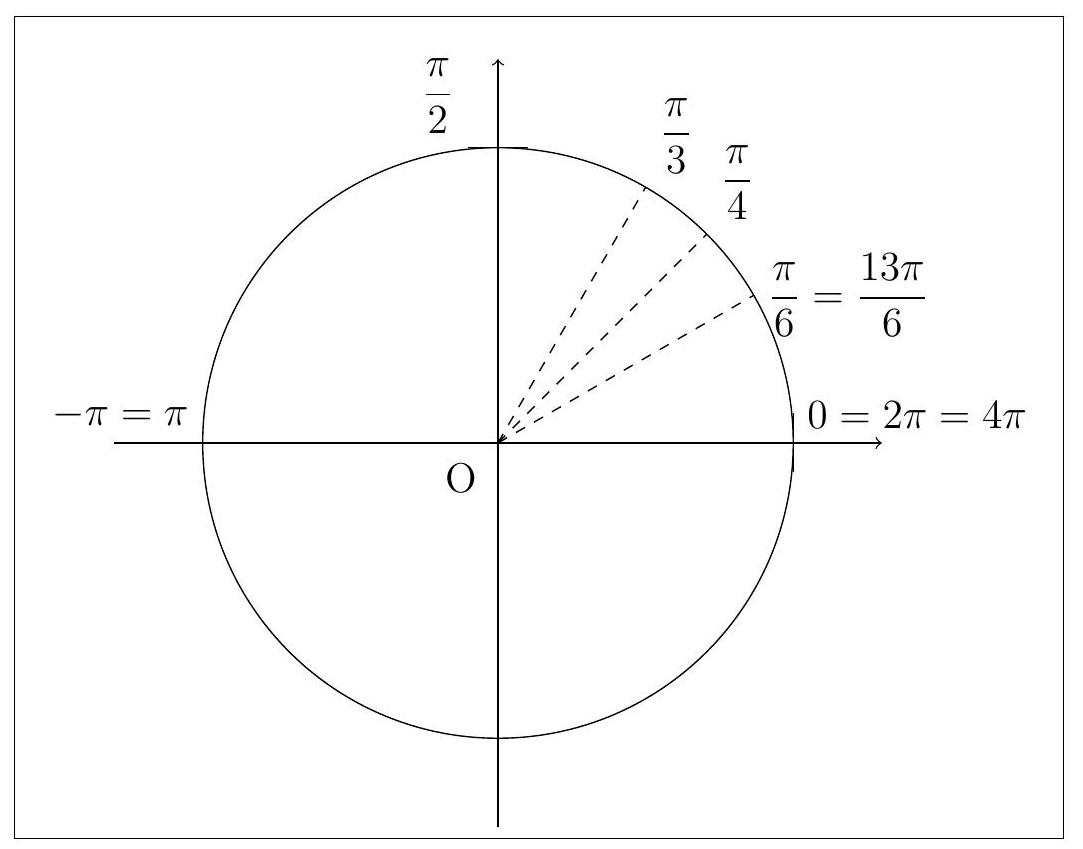
\includegraphics[width=0.6\textwidth, center]{2024_12_30_08b7afd589db230261ebg-03}
\end{remark}

\begin{method}{Déterminer la mesure d'un angle en radian}{}
On utilise la proportionnalité d'un angle en radian et en degré $(180^{\circ}=\pi\ \mathrm{rad})$.
\end{method}

Exemple. Compléter le tableau suivant en donnant l'une des mesures de l'angle :

{\renewcommand{\arraystretch}{1.2}%
\begin{center}
\begin{tabular}{|c|c|c|c|c|c|c|c|c|}
\hline
Angle en degré & 0 & 30 & 45 & 60 & 90 & 180 & 270 & 360 \\
\hline
Angle en radian &  &  &  &  &  & $\pi$ &  &  \\
\hline
\end{tabular}
\end{center}
}

Solution :

{\renewcommand{\arraystretch}{2}%
\begin{center}
\begin{tabular}{|c|c|c|c|c|c|c|c|c|}
\hline
Angle en degré & 0 & 30 & 45 & 60 & 90 & 180 & 270 & 360 \\
\hline
Angle en radian & \hide{0} & \hide{$\dfrac{\pi}{6}$} & \hide{$\dfrac{\pi}{4}$} & \hide{$\dfrac{\pi}{3}$} & \hide{$\dfrac{\pi}{2}$} & $\pi$ & \hide{$\dfrac{3 \pi}{2}$} & \hide{$2 \pi$} \\[5pt]
\hline
\end{tabular}
\end{center}
}

\subsection{Mesure principale d'un angle}
\begin{definition}{}{}
Parmi toutes les mesures d'un angle, la mesure principale est celle qui appartient à \hide{$]-\pi ; \pi]$}.
\end{definition}

\begin{method}{Déterminer la mesure principale d'un angle}{}
\begin{itemize}
  \item Si la mesure de l'angle est déjà dans l'intervalle $]-\pi ; \pi]$, alors c'est la mesure principale.
  \item Si la mesure est strictement supérieure à $\pi$, on soustrait $2 \pi$ autant de fois que nécessaire pour obtenir une mesure dans $]-\pi ; \pi]$.
  \item Si la mesure est inférieure ou égale à $-\pi$, on ajoute $2 \pi$ autant de fois que nécessaire pour obtenir une mesure dans $]-\pi ; \pi]$.
\end{itemize}
\end{method}

\begin{example}
On considère un angle de mesure $\dfrac{29 \pi}{6}$. Quelle est la mesure principale de cet angle ?

~\\Solution :\\

$\dfrac{29 \pi}{6}$ n'est pas la mesure principale car $\left.\left.\dfrac{29 \pi}{6} \notin\right]-\pi ; \pi\right]$.\\
On soustrait $2 \pi$ :

\vspace{0.5em}

$\dfrac{29 \pi}{6}-2 \pi=\dfrac{29 \pi}{6}-\dfrac{12 \pi}{6}=\dfrac{17 \pi}{6}$.\\
Mais $\left.\left.\dfrac{17 \pi}{6} \notin\right]-\pi ; \pi\right]$.\\
On soustrait donc de nouveau $2 \pi$.

\vspace{0.5em}

$\dfrac{17 \pi}{6}-2 \pi=\dfrac{17 \pi}{6}-\dfrac{12 \pi}{6}=\dfrac{5 \pi}{6}$.\\

\vspace{0.5em}

Comme $\left.\left.\dfrac{5 \pi}{6} \in\right]-\pi ; \pi\right]$, la mesure principale de l'angle est de $\dfrac{5 \pi}{6}$.
\end{example}

\subsection{Angle orienté entre deux vecteurs}
\begin{definition}{}{}
Soient $\vec{u}$ et $\vec{v}$ deux vecteurs non nuls. Soient M et N les points tels que $\overrightarrow{\mathrm{OM}}$ et $\overrightarrow{\mathrm{ON}}$ sont les représentants respectifs de $\vec{u}$ et $\vec{v}$ d'origine O. Soient M' et N' les points d'intersection des demi-droites [OM) et [ON) avec le cercle trigonométrique. Une mesure de l'angle orienté entre $\vec{u}$ et $\vec{v}$, noté $(\vec{u} ; \vec{v})$, est définie comme étant une mesure de l'angle au centre $\hideM{\widehat{\mathrm{M}^{\prime} \mathrm{ON}^{\prime}}}$.
\end{definition}

\begin{remark}
\begin{itemize}
  \item[]
  \item Si M est le point image du réel $x$, alors $(\overrightarrow{\mathrm{OI}} ; \overrightarrow{\mathrm{OM}})=x$.
  \item Tout comme les angles définis sur le cercle trigonométrique, un angle orienté entre deux vecteurs a une infinité de mesures différentes.\\
\end{itemize}
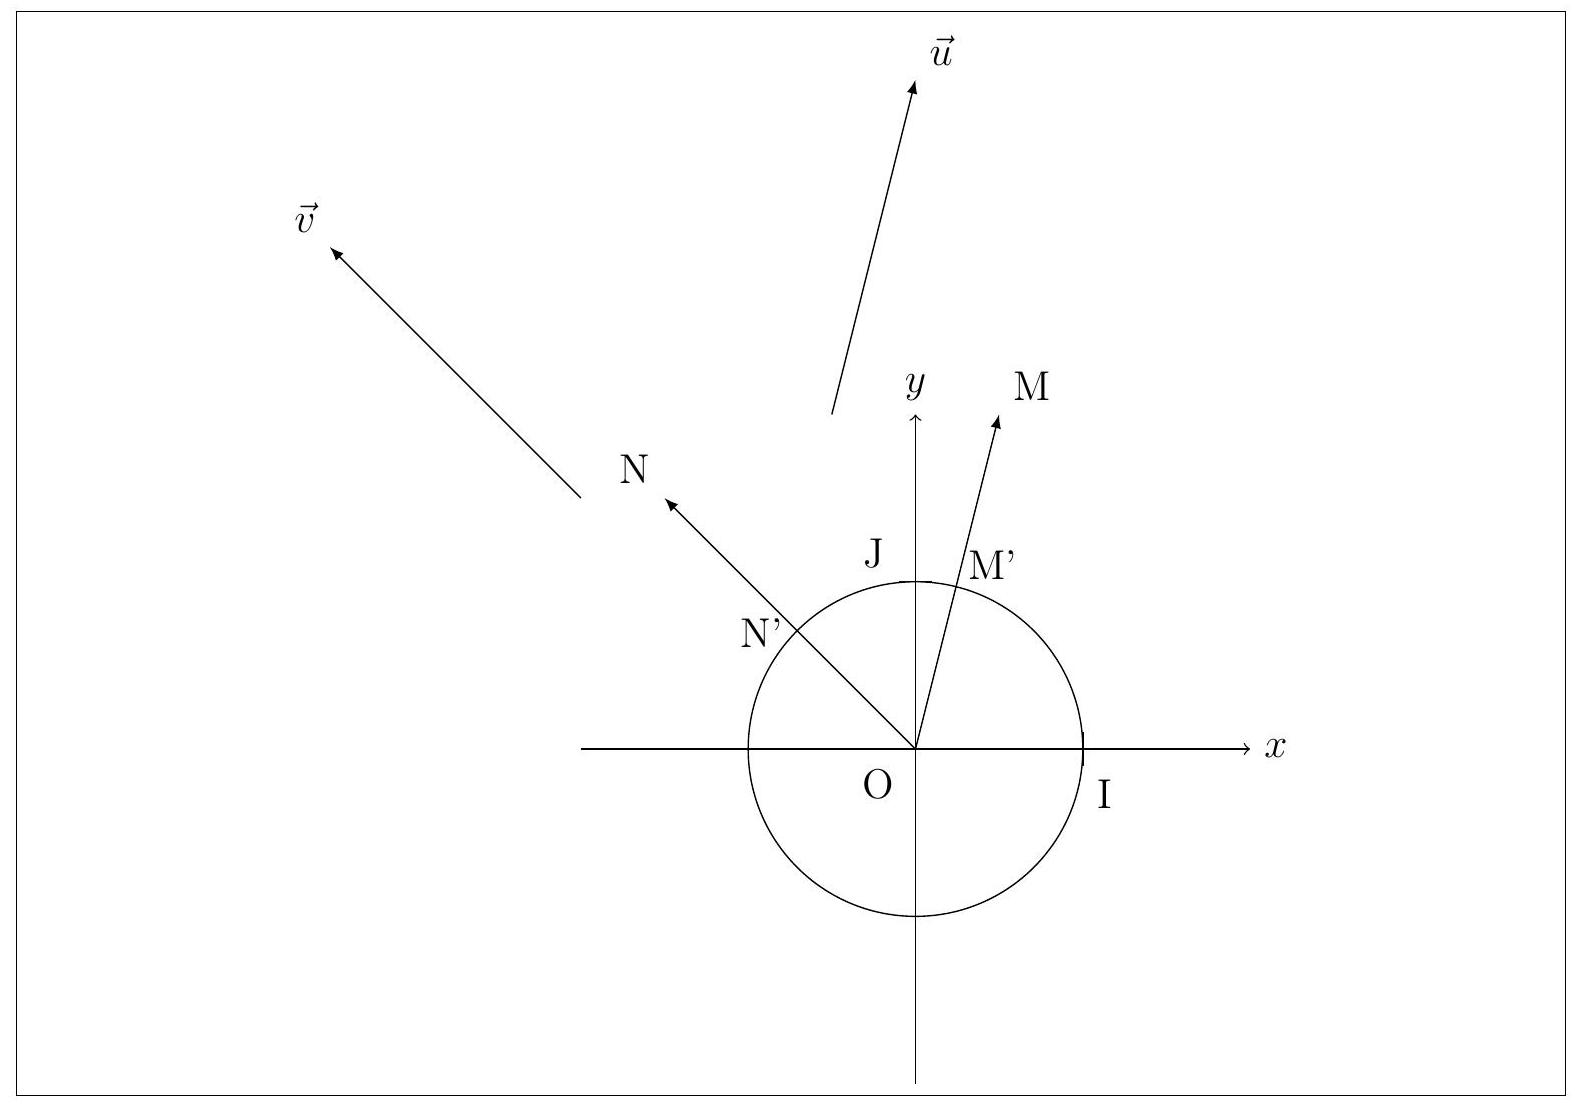
\includegraphics[width=0.9\textwidth, center]{2024_12_30_08b7afd589db230261ebg-05}
\end{remark}

\newpage

\section{Cosinus et sinus d'un nombre réel}
\subsection{Rappel : cosinus et sinus dans un triangle rectangle}

\begin{center}
\fbox{\begin{minipage}{0.85\textwidth}
  
\begin{center}
  \textbf{Introduction de la notion de cosinus}
\end{center}

On considère deux triangles ABC et $\mathrm{A}^{\prime} \mathrm{B}^{\prime} \mathrm{C}^{\prime}$ qui sont rectangles respectivement en B et en $\mathrm{B}^{\prime}$ et tels que $\widehat{\mathrm{B}^{\prime} \mathrm{A}^{\prime} \mathrm{C}}=\widehat{\mathrm{BAC}}$. Quitte à effectuer un déplacement de ces triangles, on peut les disposer comme sur le dessin ci-dessous.

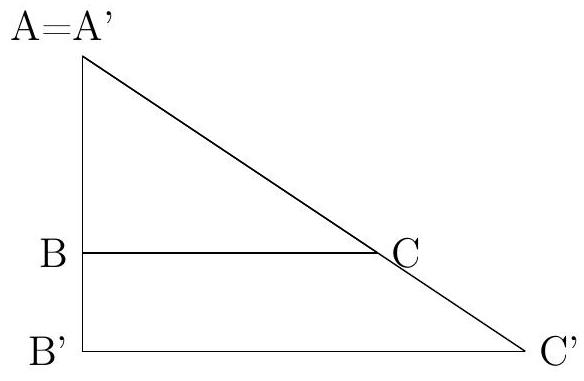
\includegraphics[width=0.4\textwidth, center]{2024_12_30_08b7afd589db230261ebg-06(1)}

D'après le théorème de Thalès, on voit alors que

$$
\dfrac{\mathrm{AB}}{\mathrm{AB}^{\prime}}=\dfrac{\mathrm{AC}}{\mathrm{AC}}
$$

Par conséquent, $\mathrm{AB} \times \mathrm{AC}^{\prime}=\mathrm{AB}^{\prime} \times \mathrm{AC}$\\
Donc $\dfrac{\mathrm{AB}}{\mathrm{AC}}=\dfrac{\mathrm{AB}^{\prime}}{\mathrm{AC}}$.\\
Finalement, cela signifie que la $\dfrac{\text { quantité côté adjacent à l'angle }}{\text { hypothénuse }}$ est la même pour les deux triangles. Par suite, cette quantité serait également la même pour tous les triangles rectangles ayant un angle égal à $\widehat{\mathrm{BAC}}$.\\
On note $\cos \left(\widehat{\mathrm{BAC}}\right)$ cette quantité.

\end{minipage}}
\end{center}

\noindent
\begin{minipage}{.7\textwidth}
\begin{definition}{}{}
Dans un triangle $A B C$ rectangle en $B$, on a :

\begin{itemize}
  \item $\cos (\widehat{\mathrm{BAC}})=\hideM{\dfrac{\mathrm{AB}}{\mathrm{AC}}}$\vspace{3pt}
  \item $\sin (\widehat{\mathrm{BAC}})=\hideM{\dfrac{\mathrm{BC}}{\mathrm{AC}}}$\vspace{3pt}
  \item $\tan (\widehat{\mathrm{BAC}})=\hideM{\dfrac{\mathrm{BC}}{\mathrm{AB}}}$
\end{itemize}
\end{definition}
\end{minipage}
\hspace{1em}
\begin{minipage}{0.25\textwidth}
\fbox{\hspace{10pt}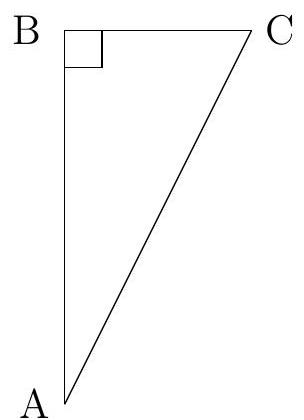
\includegraphics[width=0.7\textwidth, center]{2024_12_30_08b7afd589db230261ebg-06}\hspace{10pt}}
\end{minipage}

\newpage

\begin{proposition}{}{}
Dans un triangle $A B C$ rectangle en $B$ :

$$
\tan (\widehat{\mathrm{BAC}})=\hideM{\frac{\sin (\widehat{\mathrm{BAC}})}{\cos (\widehat{\mathrm{BAC}})}}
$$\vspace{1pt}

\end{proposition}

\begin{demo}
On considère un triangle ABC rectangle en B . On a alors :

$$
\frac{\sin (\widehat{\mathrm{BAC}})}{\cos (\widehat{\mathrm{BAC}})}=\frac{\frac{\mathrm{BC}}{\mathrm{AC}}}{\frac{\mathrm{AB}}{\mathrm{AC}}}=\frac{\mathrm{BC}}{\mathrm{AC}} \times \frac{\mathrm{AC}}{\mathrm{AB}}=\frac{\mathrm{BC}}{\mathrm{AB}}=\tan (\widehat{\mathrm{BAC}})
$$
\end{demo}

\begin{proposition}{}{}
Dans un triangle ABC rectangle en B :

$$
(\sin (\widehat{\mathrm{BAC}}))^{2}+(\cos (\widehat{\mathrm{BAC}}))^{2}=\hideM{1}
$$
\end{proposition}

\begin{remark}
En général, on note $\sin ^{2}(\widehat{\mathrm{BAC}})+\cos ^{2}(\widehat{\mathrm{BAC}})=1$.
\end{remark}

\begin{demo}
On considère un triangle ABC rectangle en B . On a alors :

$$
\begin{aligned}
(\sin (\widehat{\mathrm{BAC}}))^{2}+(\cos (\widehat{\mathrm{BAC}}))^{2} & =\left(\frac{\mathrm{BC}}{\mathrm{AC}}\right)^{2}+\left(\frac{\mathrm{AB}}{\mathrm{AC}}\right)^{2} \\
& =\frac{\mathrm{BC}^{2}}{\mathrm{AC}^{2}}+\frac{\mathrm{AB}^{2}}{\mathrm{AC}^{2}} \\
& =\frac{\mathrm{BC}^{2}+\mathrm{AB}^{2}}{\mathrm{AC}^{2}} \\
& =\frac{\mathrm{AC}^{2}}{\mathrm{AC}^{2}}\left(\text {car d'après Pythagore, } \mathrm{BC}^{2}+\mathrm{AB}^{2}=\mathrm{AC}^{2}\right) \\
& =1
\end{aligned}
$$
\end{demo}

\newpage
\subsection{Définition du cosinus et du sinus d'un nombre réel}
\begin{definition}{}{}
Soit $x \in \mathbb{R}$ et $M$ le point image de $x$ sur le cercle trigonométrique.

\begin{itemize}
  \item L'abscisse du point $M$ est appelée \hide{cosinus} de $x$. On la note \hide{$\cos (x)$}.
  \item L'ordonnée du point $M$ est appelée \hide{sinus} de $x$. On la note \hide{$\sin (x)$}.
\end{itemize}
\end{definition}
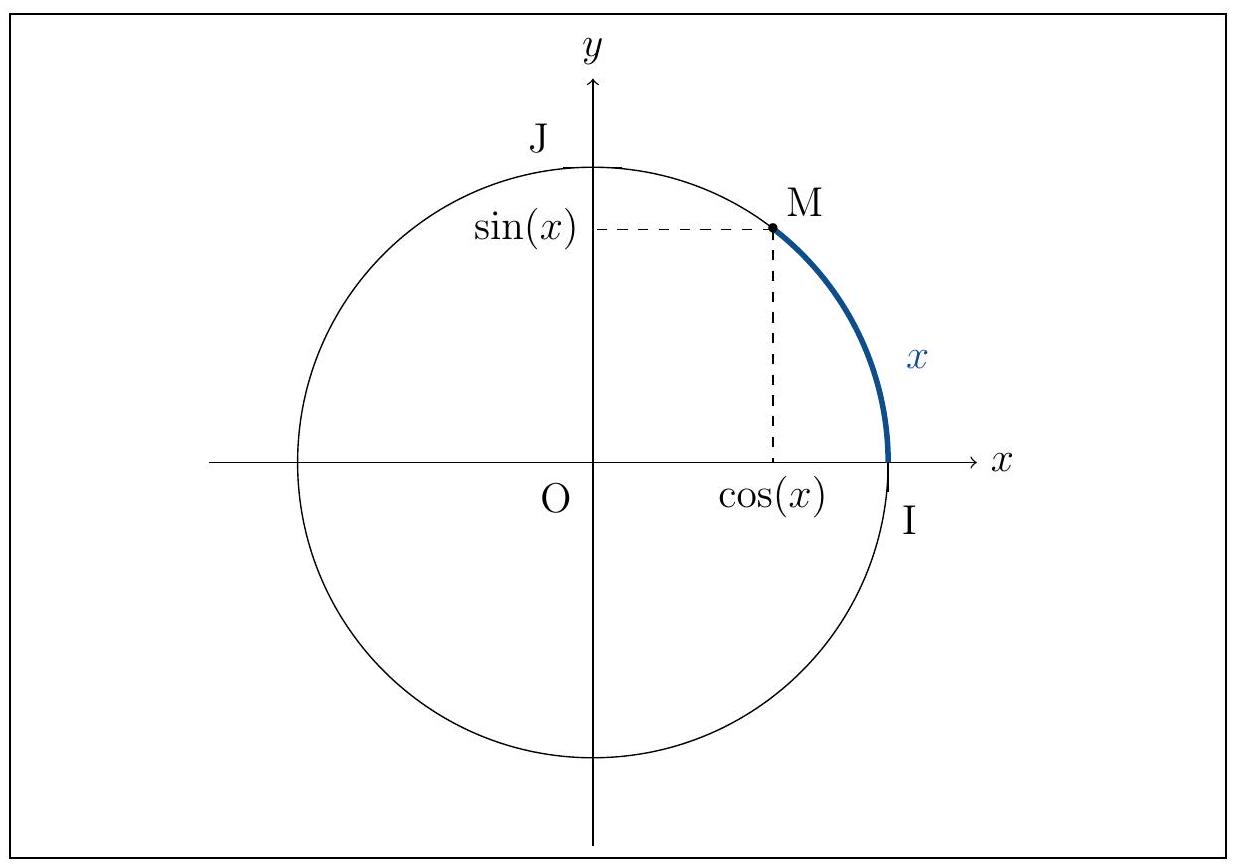
\includegraphics[width=0.75\textwidth, center]{2024_12_30_08b7afd589db230261ebg-08}

\begin{remark}
Cette définition généralise la notion de cosinus et de sinus car, dans le cas d'un angle aigu, les définitions 6 et 7 coïncident.\\
En effet, si on note H le projeté orthogonal de M sur l'axe des abscisses, on obtient, dans le triangle rectangle OHM :

$$
\cos (\widehat{\mathrm{HOM}})=\frac{\mathrm{OH}}{\mathrm{OM}}=\mathrm{OH} \quad(\operatorname{car} \mathrm{OM}=1)
$$
\end{remark}

\begin{proposition}{}{}
Pour tout $x \in \mathbb{R}$,

\begin{itemize}
  \item $-1 \leqslant \hideM{\cos (x)} \leqslant 1$
  \item $-1 \leqslant \hideM{\sin (x)} \leqslant 1$
  \item $\cos ^{2}(x)+\sin ^{2}(x)=\hideM{1}$
\end{itemize}
\end{proposition}

\begin{demo}
Les deux premiers points découlent directement du fait que $\cos (x)$ et $\sin (x)$ sont les abscisses et ordonnées d'un point du cercle trigonométrique (de rayon 1). Le dernier point est une conséquence immédiate de la propriété 3.
\end{demo}

\subsection{Formules des angles associés}
\begin{proposition}{}{}
Pour tout $x \in \mathbb{R}$ :

\begin{itemize}
  \item $\cos (-x)=\hideM{\cos (x)}$
  \item $\sin (-x)=\hideM{-\sin (x)}$
\end{itemize}
\end{proposition}
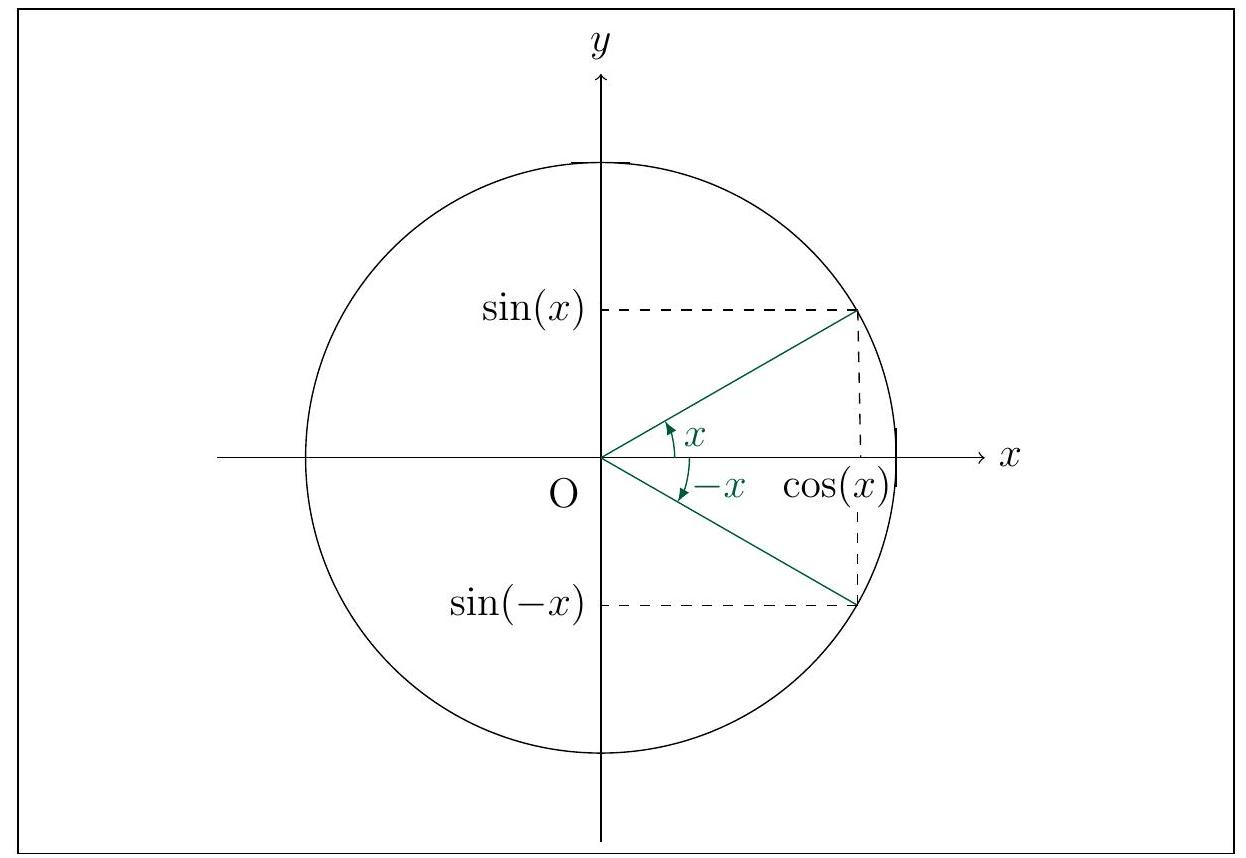
\includegraphics[width=0.65\textwidth, center]{2024_12_30_08b7afd589db230261ebg-09(1)}

\begin{proposition}{}{}
Pour tout $x \in \mathbb{R}$ :

\begin{itemize}
  \item $\cos (\pi-x)=\hideM{-\cos (x)}$
  \item $\sin (\pi-x)=\hideM{\sin (x)}$
\end{itemize}
\end{proposition}
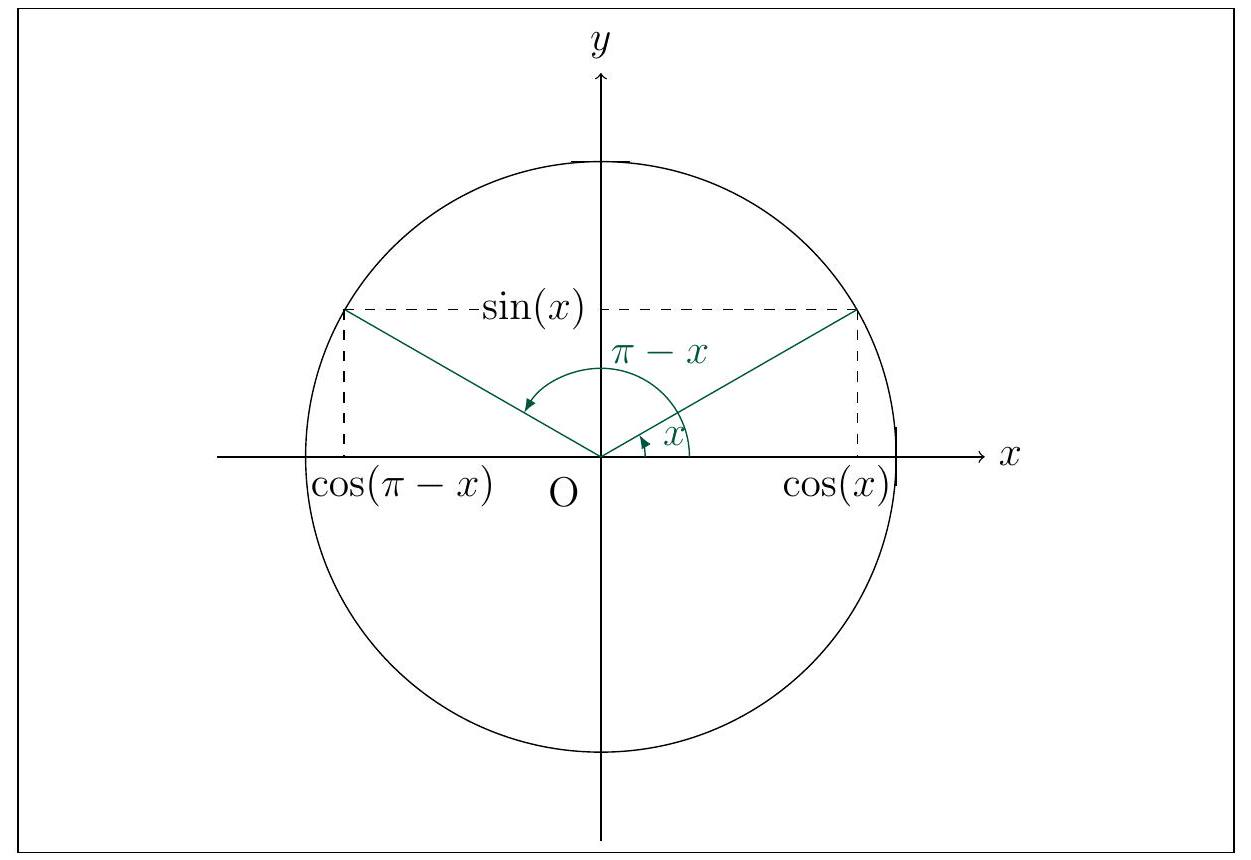
\includegraphics[width=0.65\textwidth, center]{2024_12_30_08b7afd589db230261ebg-09}

\begin{proposition}{}{}
Pour tout $x \in \mathbb{R}$ :

\begin{itemize}
  \item $\cos (\pi+x)=\hideM{-\cos (x)}$
  \item $\sin (\pi+x)=\hideM{-\sin (x)}$
\end{itemize}
\end{proposition}
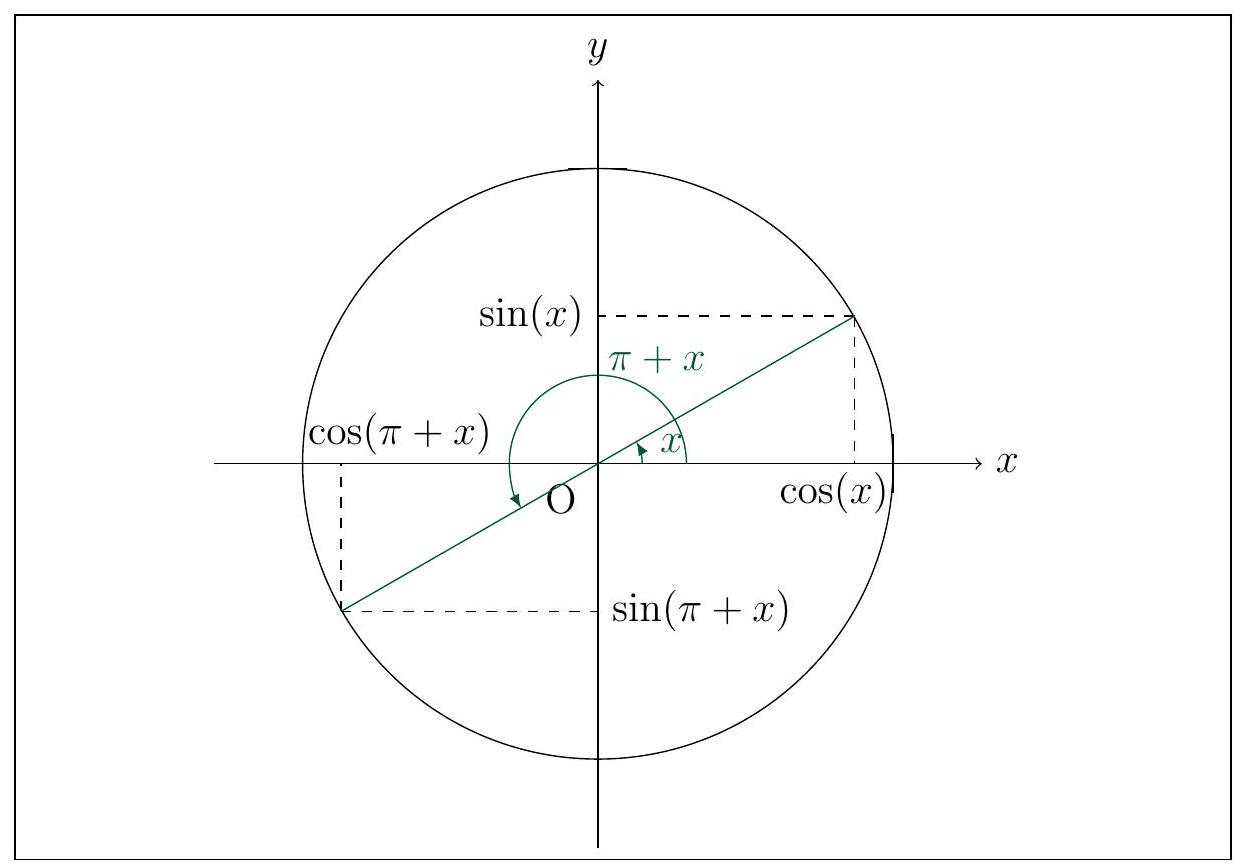
\includegraphics[width=0.65\textwidth, center]{2024_12_30_08b7afd589db230261ebg-10}

\begin{proposition}{}{}
Pour tout $x \in \mathbb{R}$ :

\begin{itemize}
  \item $\cos \left(\frac{\pi}{2}-x\right)=\hideM{\sin (x)}$
  \item $\sin \left(\frac{\pi}{2}-x\right)=\hideM{\cos (x)}$
\end{itemize}
\end{proposition}
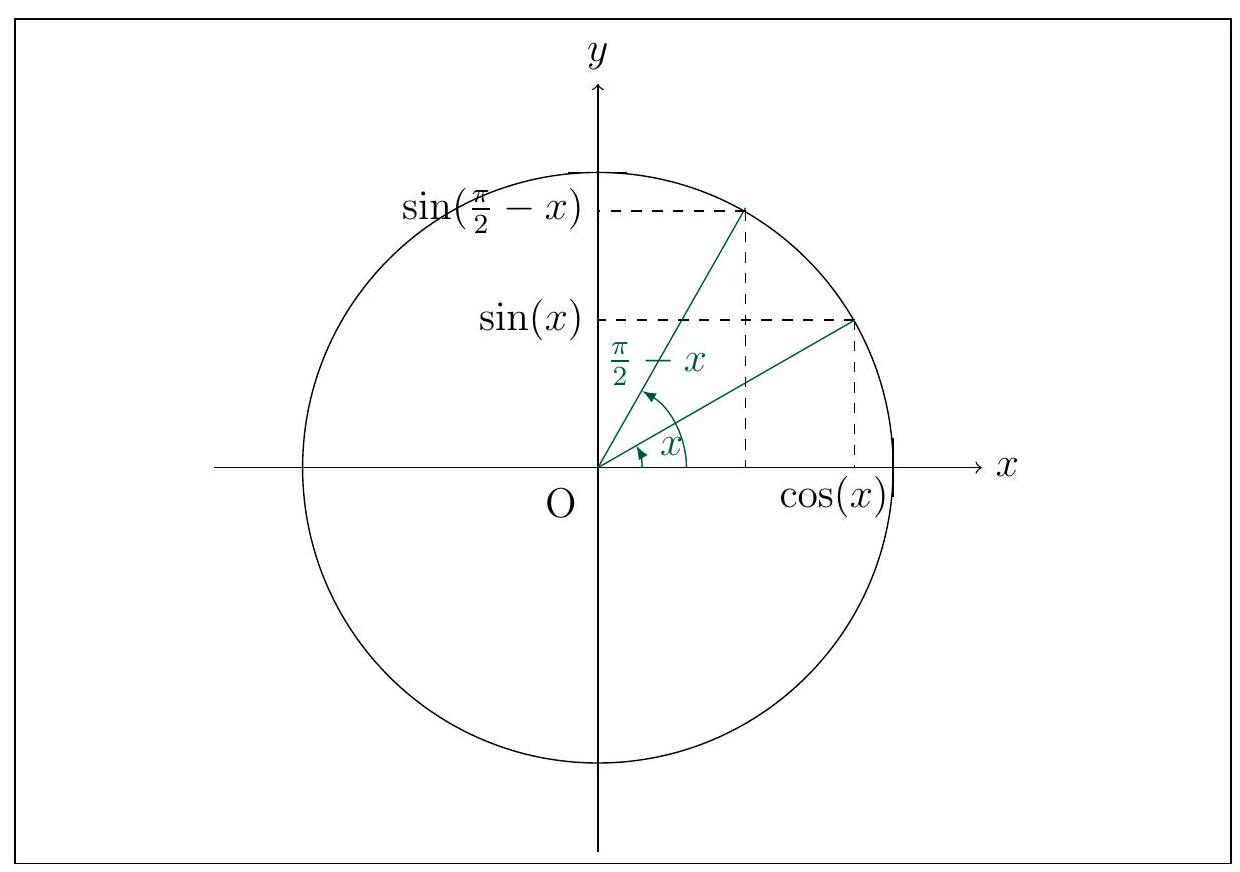
\includegraphics[width=0.65\textwidth, center]{2024_12_30_08b7afd589db230261ebg-10(1)}

\begin{proposition}{}{}
Pour tout $x \in \mathbb{R}$ :

\begin{itemize}
  \item $\cos \left(\frac{\pi}{2}+x\right)=\hideM{-\sin (x)}$
  \item $\sin \left(\frac{\pi}{2}+x\right)=\hideM{\cos (x)}$
\end{itemize}
\end{proposition}
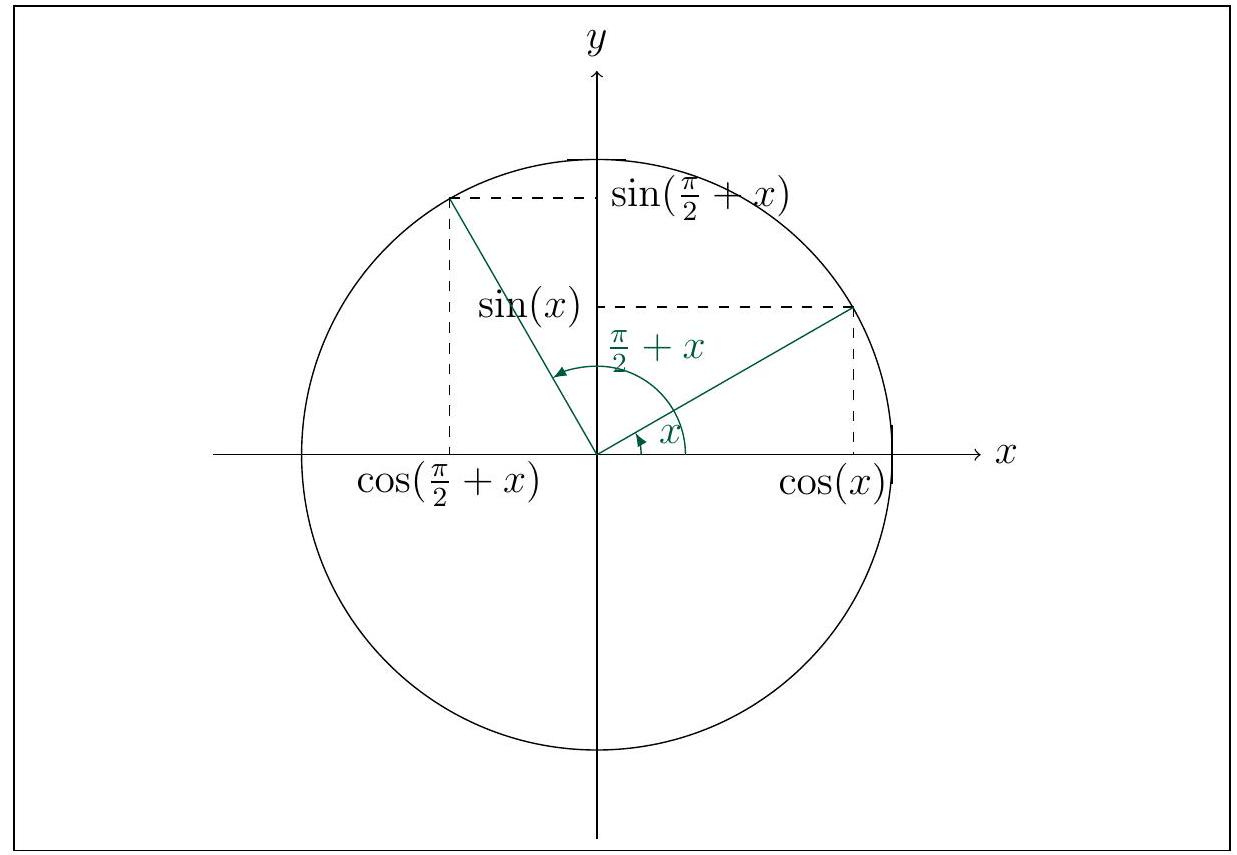
\includegraphics[width=0.65\textwidth, center]{2024_12_30_08b7afd589db230261ebg-11}

\begin{remark}
Les propriétés des angles associés (propriétés ci-dessus) ne sont pas à connaître par coeur mais doivent pouvoir être retrouvées très rapidement en faisant un dessin.
\end{remark}

\newpage

\subsection{Valeurs remarquables}
Les valeurs ci-dessous sont à connaître :

\begin{proposition}{}{}
\begin{center}

{\renewcommand{\arraystretch}{3}%
\begin{tabular}{|c|c|c|c|c|c|c|}
\hline
$x$ & 0 & $\dfrac{\pi}{6}$ & $\dfrac{\pi}{4}$ & $\dfrac{\pi}{3}$ & $\dfrac{\pi}{2}$ & $\pi$ \\
\hline
$\cos(x)$ & \hideM{1} & \hide{$\dfrac{\sqrt{3}}{2}$} & \hide{$\dfrac{\sqrt{2}}{2}$} & \hide{$\dfrac{1}{2}$} & \hide{0} & \hide{-1} \\
\hline
$\sin (x)$ & \hide{0} & \hide{$\dfrac{1}{2}$} & \hide{$\dfrac{\sqrt{2}}{2}$} & \hide{$\dfrac{\sqrt{3}}{2}$} & \hide{1} & \hide{0} \\
\hline
\end{tabular}
}
\end{center}
\end{proposition}

\begin{center}
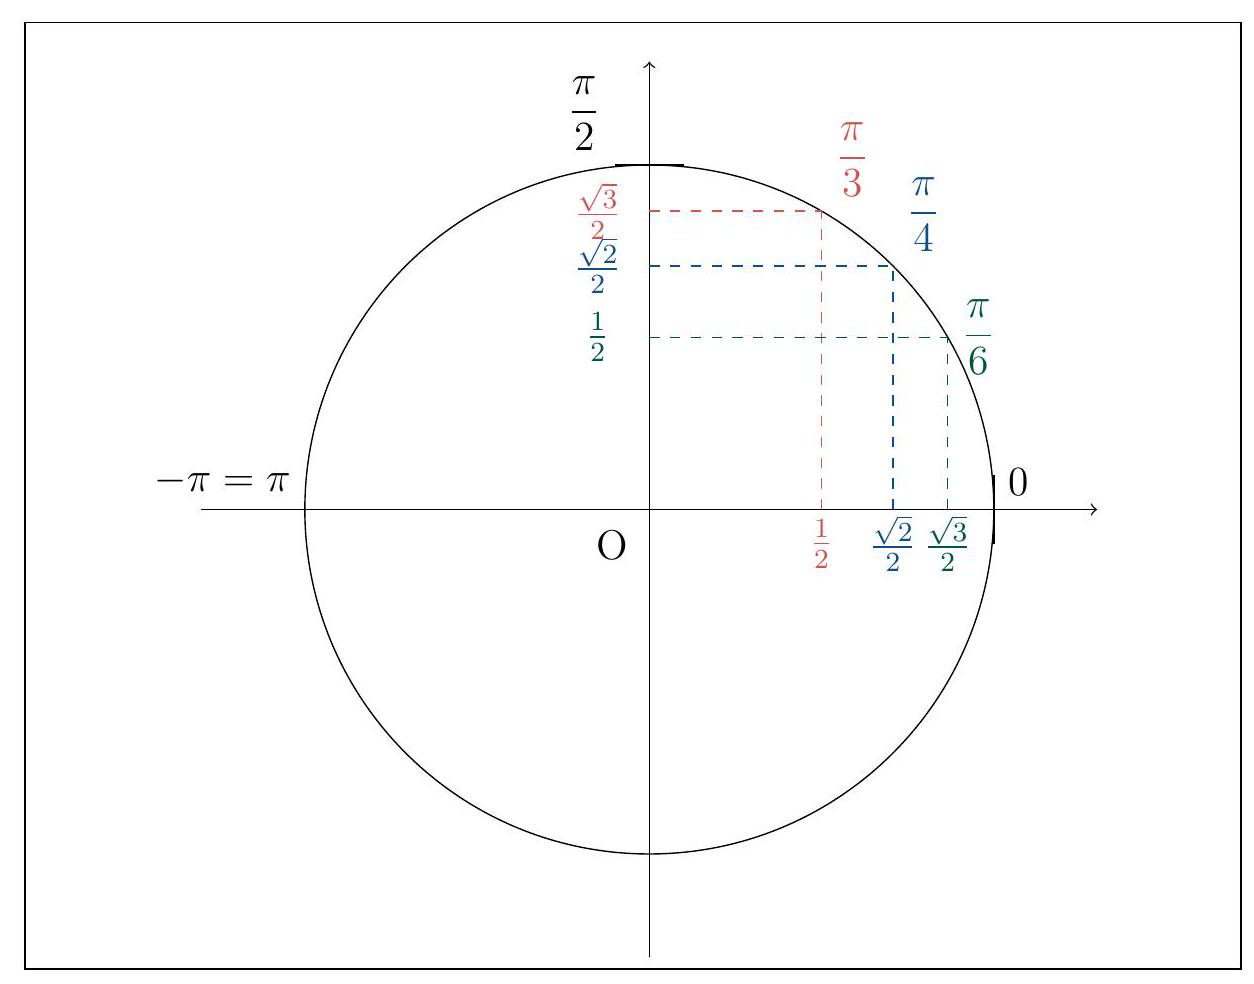
\includegraphics[width=0.8\textwidth]{2024_12_30_08b7afd589db230261ebg-12}
\end{center}

\begin{demo}
\begin{itemize}
  \item Les valeurs de $\cos (0), \sin (0), \cos (\pi), \sin (\pi), \cos \left(\dfrac{\pi}{2}\right)$ et $\sin \left(\dfrac{\pi}{2}\right)$ se lisent directement sur le cercle trigonométrique.
  \newpage
  \item Montrons que $\cos \left(\dfrac{\pi}{4}\right)=\dfrac{\sqrt{2}}{2}$ et $\sin \left(\dfrac{\pi}{4}\right)=\dfrac{\sqrt{2}}{2}$.

On considère le point M sur le cercle trigonométrique tel que $\widehat{\mathrm{IOM}}=\dfrac{\pi}{4}$ puis le point H , projeté orthogonal de M sur (OI) et le point H', projeté orthogonal de M sur (OJ).\\
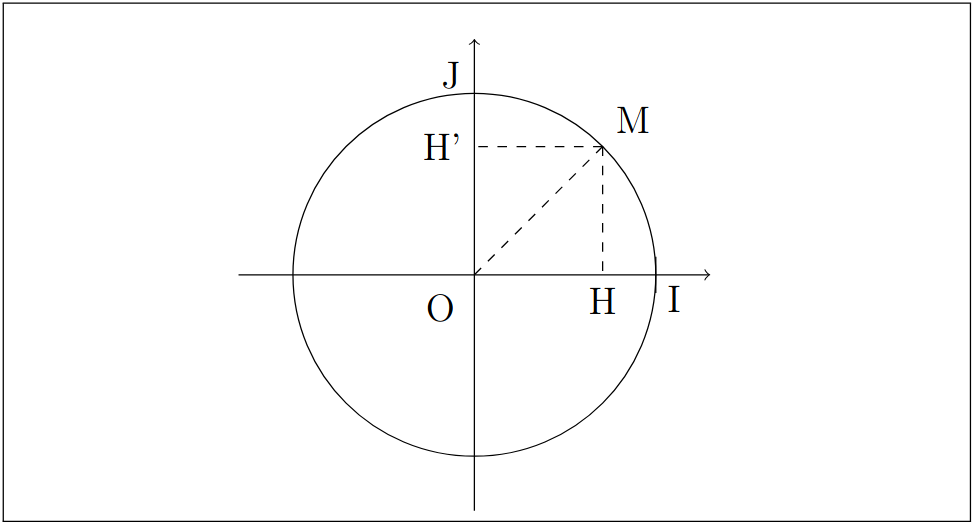
\includegraphics[width=0.7\linewidth, center]{swappy-20241230_125534.png}

La somme des angles d'un triangle est égale à $\pi$ rad donc, dans le triangle OMH,

$$
\widehat{\mathrm{OMH}}=\pi-\dfrac{\pi}{4}-\dfrac{\pi}{2}=\dfrac{\pi}{4}
$$

Ainsi, le triangle OMH a deux angles égaux donc il est isocèle et donc $\mathrm{OH}=\mathrm{HM}$. De plus, d'après le théorème de Pythagore dans OHM :

$$
\begin{aligned}
\mathrm{OM}^{2} & =\mathrm{HM}^{2}+\mathrm{OH}^{2} \\
& =2 \mathrm{OH}^{2}(\operatorname{car~OH}=\mathrm{HM}) \\
\text { donc } \quad \mathrm{OM} & =\sqrt{2} \times \mathrm{OH}
\end{aligned}
$$

Finalement, on en déduit que :

$$
\begin{aligned}
\mathrm{OH} & =\dfrac{1}{\sqrt{2}} O M \\
& =\dfrac{1}{\sqrt{2}}\ (\operatorname{car} \mathrm{OM}=1) \\
& =\dfrac{1 \times \sqrt{2}}{\sqrt{2} \times \sqrt{2}}=\dfrac{\sqrt{2}}{2}
\end{aligned}
$$

Par définition du cosinus d'un angle, on voit que $\cos \left(\dfrac{\pi}{4}\right)=\mathrm{OH}=\dfrac{\sqrt{2}}{2}$.\\
Enfin, sachant que OHMH' est un carré, on en déduit que $\sin \left(\dfrac{\pi}{4}\right)=\mathrm{OH}^{\prime}=\mathrm{OH}=\dfrac{\sqrt{2}}{2}$.
\newpage

  \item Montrons que $\cos \left(\dfrac{\pi}{3}\right)=\dfrac{1}{2}$ et $\sin \left(\dfrac{\pi}{3}\right)=\dfrac{\sqrt{3}}{2}$.

On considère le point M sur le cercle trigonométrique tel que $\widehat{\mathrm{IOM}}=\dfrac{\pi}{3}$.\\
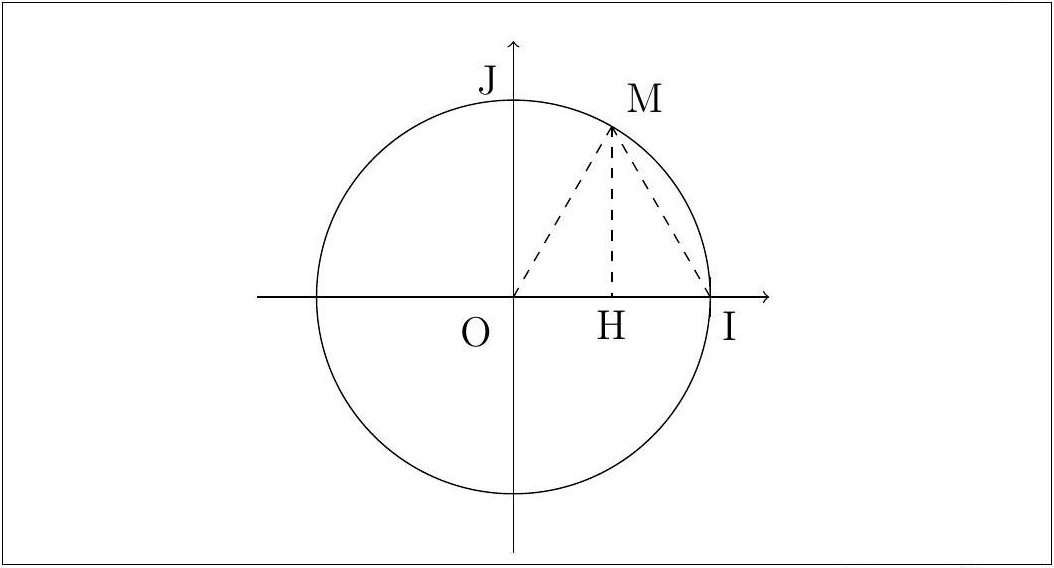
\includegraphics[width=0.7\linewidth, center]{2024_12_30_08b7afd589db230261ebg-14}

Comme $\mathrm{OM}=\mathrm{OI}=1$, le triangle IOM est isocèle puis comme $\widehat{\mathrm{IOM}}=\dfrac{\pi}{3}$, on en déduit que IOM est équilatéral.\\
On considère le point H , projeté orthogonal de M sur (OI). Comme les médiatrices et les hauteurs d'un triangle équilatéral sont confondues, on en déduit que (HM) est la médiatrice de $[O I]$ et donc que :

$$
\cos \left(\dfrac{\pi}{3}\right)=\mathrm{OH}=\dfrac{1}{2}
$$

Ensuite, en utilisant le théorème de Pythagore dans le triangle OHM, on obtient :

$$
\mathrm{OM}^{2}=\mathrm{OH}^{2}+\mathrm{HM}^{2}
$$

Par conséquent :

$$
\begin{aligned}
\mathrm{HM} & =\sqrt{\mathrm{OM}^{2}-\mathrm{OH}^{2}} \quad \text { car } \mathrm{HM}>0 \\
& =\sqrt{1^{2}-\left(\dfrac{1}{2}\right)^{2}} \\
& =\sqrt{1-\dfrac{1}{4}}=\sqrt{\dfrac{3}{4}}=\dfrac{\sqrt{3}}{2}
\end{aligned}
$$

  \item Montrons que $\cos \left(\dfrac{\pi}{6}\right)=\dfrac{\sqrt{3}}{2}$ et $\sin \left(\dfrac{\pi}{6}\right)=\dfrac{1}{2}$.

En fait, $\dfrac{\pi}{6}=\dfrac{\pi}{2}-\dfrac{\pi}{3}$.\\
On déduit donc les valeurs de $\cos \left(\dfrac{\pi}{6}\right)$ et $\sin \left(\dfrac{\pi}{6}\right)$ à l'aide des Propositions 8 et 9 .

\[ \begin{array}{rl}
\begin{aligned}
\cos \left(\dfrac{\pi}{6}\right) & =\cos \left(\dfrac{\pi}{2}-\dfrac{\pi}{3}\right) \\
& =\sin \left(\dfrac{\pi}{3}\right) \\
& =\dfrac{\sqrt{3}}{2}
\end{aligned} \hspace{20pt} & \hspace{20pt} \begin{aligned}
\sin \left(\dfrac{\pi}{6}\right) & =\sin \left(\dfrac{\pi}{2}-\dfrac{\pi}{3}\right) \\
& =\cos \left(\dfrac{\pi}{3}\right) \\
& =\dfrac{1}{2}
\end{aligned}
\end{array}
\]
\end{itemize}
\end{demo}


\begin{method}{Déterminer le cosinus ou le sinus d'un nombre réel}{}
\begin{itemize}
  \item Faire un dessin : placer l'angle en question sur le cercle.
  \item Extraire du tableau ci-dessus les valeurs dont l'angle a le même dénominateur que celui considéré.
  \item Utiliser les formules des angles associées pour relier le cosinus ou le sinus recherché avec les valeurs du tableau.
\end{itemize}
\end{method}

\noindent
\begin{example}
Déterminer $\cos \left(\dfrac{3 \pi}{4}\right)$.

\begin{minipage}{.5\textwidth}
~\\Solution :\\
On sait que $\cos \left(\dfrac{\pi}{4}\right)=\dfrac{\sqrt{2}}{2}$.\\
D'après le dessin ci-contre, on en déduit que :

$$
\cos \left(\dfrac{3 \pi}{4}\right)=-\dfrac{\sqrt{2}}{2}
$$
\end{minipage}
\begin{minipage}{0.5\textwidth}
%\fbox{\hspace{10pt}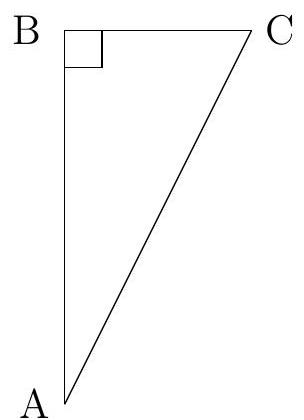
\includegraphics[width=0.7\textwidth, center]{2024_12_30_08b7afd589db230261ebg-06}\hspace{10pt}}
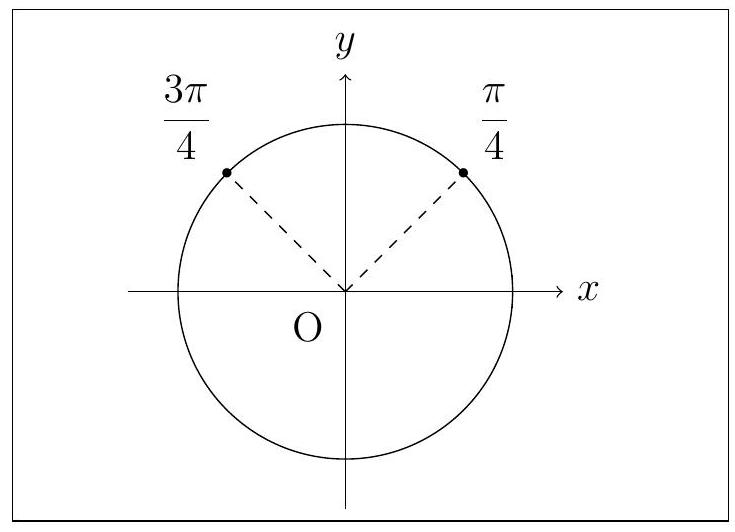
\includegraphics[width=1\textwidth]{2024_12_30_08b7afd589db230261ebg-15}
\end{minipage}
\end{example}

\begin{savoir}{}{}
\begin{itemize}
  \item Convertir des degrés en radians et inversement.
  \item Déterminer la mesure principale d'un angle.
  \item Placer un point sur le cercle trigonométrique.
  \item Déterminer le cosinus et le sinus d'un nombre réel.
\end{itemize}
\end{savoir}

\end{document}